\documentclass[aspectratio=169]{beamer}
\usepackage[UTF8]{ctex}
\usepackage{amsmath, amssymb, amsfonts}
\usepackage{tikz}
\usepackage{graphicx}
\usepackage{animate}
\usepackage{xcolor}

\usefonttheme{professionalfonts}
\usefonttheme{serif}
\usepackage{fontspec}
\setmainfont{Noto Serif CJK SC}
\setsansfont{Noto Sans CJK SC}
\setmonofont{Noto Sans Mono CJK SC}

% Define colors
\definecolor{myblue}{RGB}{0, 102, 204}
\definecolor{mygreen}{RGB}{0, 153, 0}
\definecolor{myred}{RGB}{204, 0, 0}

% Beamer theme settings
\usetheme{Madrid}
\usecolortheme{default}
\setbeamercolor{structure}{fg=myblue}

% Title page information
\title[计算图与反向传播]{计算图、反向传播与梯度下降\\初学者指南}
\subtitle{从基础概念到实际应用}
\author{Anson}
\institute{深度学习社}
\date{\today}

\begin{document}

% Title slide
\begin{frame}
\titlepage
\small{Cooperated with Kimi AI}
\end{frame}

% Table of contents
\begin{frame}{目录}
    \begin{columns}
        \column{0.4\textwidth}
        \tableofcontents
        \column{0.4\textwidth}
        \includegraphics[width=\textwidth]{images/computational_diagram.png}
    \end{columns}
\end{frame}

\section{引言:什么是机器学习?}

\begin{frame}{什么是机器学习?}
\begin{block}{简单定义}
机器学习是让计算机\alert{从数据中学习},而不需要明确编程每一个规则。
\end{block}

\begin{exampleblock}{生活中的例子}
\begin{itemize}
    \item 垃圾邮件过滤
    \item 推荐系统(Netflix、淘宝)
    \item 语音识别
    \item 图像识别
\end{itemize}
\end{exampleblock}

\begin{alertblock}{关键问题}
如何\alert{自动调整}模型的参数,使其表现更好?
\end{alertblock}
\end{frame}

\begin{frame}{为什么需要计算图和反向传播?}
\begin{itemize}
    \item 现代机器学习模型(如神经网络)非常复杂
    \item 需要高效的计算方法来训练这些模型
    \item 计算图提供了清晰的数学框架
    \item 反向传播让我们能够高效地计算梯度
    \item 梯度下降帮助我们找到最优参数
\end{itemize}

\begin{center}
\large
\hfill
\alert{今天我们将学习这三个核心概念!}
\end{center}
\end{frame}

\section{计算图基础}

\begin{frame}{什么是计算图?}
\begin{block}{直观理解}
计算图就是把\alert{数学表达式}画成\alert{图}的形式,让我们更容易理解和计算。
\end{block}

\begin{exampleblock}{简单例子:计算 $f(x,y) = (x+y) \times y$}
\begin{center}
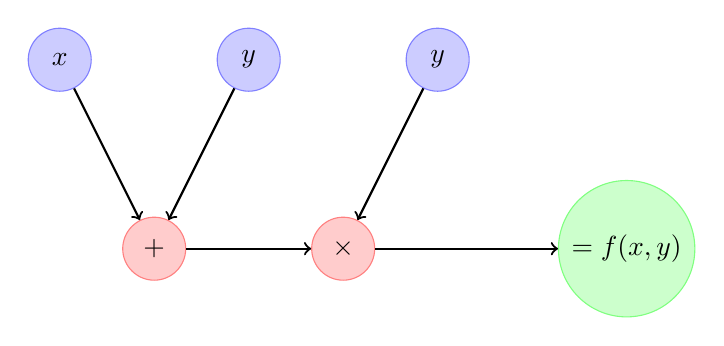
\begin{tikzpicture}[scale=1.2]
    % Nodes
    \node[circle, draw=blue!50, fill=blue!20, minimum size=0.8cm] (x) at (0,2) {$x$};
    \node[circle, draw=blue!50, fill=blue!20, minimum size=0.8cm] (y1) at (2,2) {$y$};
    \node[circle, draw=blue!50, fill=blue!20, minimum size=0.8cm] (y2) at (4,2) {$y$};
    
    % Operation nodes
    \node[circle, draw=red!50, fill=red!20, minimum size=0.8cm] (plus) at (1,0) {$+$};
    \node[circle, draw=red!50, fill=red!20, minimum size=0.8cm] (times) at (3,0) {$\times$};
    
     % Result
    \node[circle, draw=green!50, fill=green!20, minimum size=1cm] (result) at (6,0) {$= f(x,y)$};

    % Edges
    \draw[->, thick] (x) -- (plus);
    \draw[->, thick] (y1) -- (plus);
    \draw[->, thick] (plus) -- (times);
    \draw[->, thick] (y2) -- (times);
    \draw[->, thick] (times) -- (result);
   
\end{tikzpicture}
\end{center}
\end{exampleblock}
\end{frame}

\begin{frame}{计算图的基本元素}

\begin{columns}[t]
\column{0.4\textwidth}
\begin{block}{节点(Nodes)}
\begin{itemize}
    \item \textcolor{blue}{输入节点}:变量或常数
    \item \textcolor{red}{操作节点}:数学运算
    \item 每个节点代表一个计算步骤
\end{itemize}
\end{block}

\column{0.55\textwidth}
\begin{block}{边(Edges)}
\begin{itemize}
    \item 表示数据流动方向
    \item 从前一个节点的输出到后一个节点的输入
    \item 帮助追踪计算的依赖关系
\end{itemize}
\end{block}
\end{columns}

\begin{exampleblock}{为什么使用计算图?}
\begin{itemize}
    \item \alert{清晰}:直观展示计算过程
    \item \alert{灵活}:容易修改和扩展
    \item \alert{高效}:便于自动求导
    \item \alert{通用}:适用于各种机器学习模型
\end{itemize}
\end{exampleblock}
\end{frame}

\begin{frame}{更复杂的例子:逻辑回归}

\begin{block}{逻辑回归模型}
预测概率:$\hat{y} = \sigma(w_1x_1 + w_2x_2 + b)$,其中\alert{$\sigma(z) = \frac{1}{1+e^{-z}}$}是sigmoid函数
\end{block}

\begin{center}
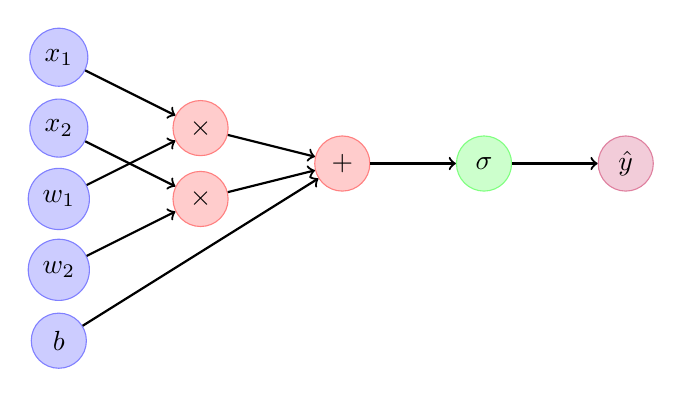
\begin{tikzpicture}[scale=0.9]
    % Input nodes
    \node[circle, draw=blue!50, fill=blue!20, minimum size=0.7cm] (x1) at (0,2) {$x_1$};
    \node[circle, draw=blue!50, fill=blue!20, minimum size=0.7cm] (x2) at (0,1) {$x_2$};
    \node[circle, draw=blue!50, fill=blue!20, minimum size=0.7cm] (w1) at (0,0) {$w_1$};
    \node[circle, draw=blue!50, fill=blue!20, minimum size=0.7cm] (w2) at (0,-1) {$w_2$};
    \node[circle, draw=blue!50, fill=blue!20, minimum size=0.7cm] (b) at (0,-2) {$b$};
    
    % Multiplication nodes
    \node[circle, draw=red!50, fill=red!20, minimum size=0.7cm] (mul1) at (2,1) {$\times$};
    \node[circle, draw=red!50, fill=red!20, minimum size=0.7cm] (mul2) at (2,0) {$\times$};
    
    % Addition
    \node[circle, draw=red!50, fill=red!20, minimum size=0.7cm] (add) at (4,0.5) {$+$};
    
    % Sigmoid
    \node[circle, draw=green!50, fill=green!20, minimum size=0.7cm] (sig) at (6,0.5) {$\sigma$};
    
    % Output
    \node[circle, draw=purple!50, fill=purple!20, minimum size=0.7cm] (y) at (8,0.5) {$\hat{y}$};
    
    % Edges
    \draw[->, thick] (x1) -- (mul1);
    \draw[->, thick] (w1) -- (mul1);
    \draw[->, thick] (x2) -- (mul2);
    \draw[->, thick] (w2) -- (mul2);
    \draw[->, thick] (mul1) -- (add);
    \draw[->, thick] (mul2) -- (add);
    \draw[->, thick] (b) -- (add);
    \draw[->, thick] (add) -- (sig);
    \draw[->, thick] (sig) -- (y);
\end{tikzpicture}
\end{center}
\end{frame}

\section{前向传播}

\begin{frame}{什么是前向传播?}
\begin{block}{直观理解}
前向传播就是\alert{从左到右}沿着计算图计算每个节点的值,直到得到最终结果。
\end{block}

\begin{exampleblock}{回忆简单例子:$f(x,y) = (x+y) \times y$}

\begin{columns}
    \column{0.4\textwidth}
假设$x=3, y=2$:
\begin{enumerate}
    \item 计算$x+y = 3+2 = 5$
    \item 计算$(x+y) \times y = 5 \times 2 = 10$
    \item 得到最终结果:$f(3,2) = 10$
\end{enumerate}

    \column{0.6\textwidth}

\begin{center}
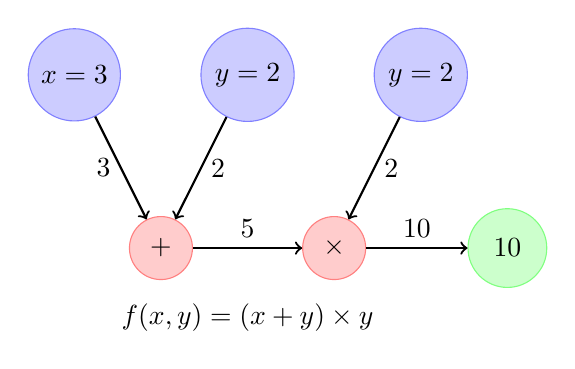
\begin{tikzpicture}[scale=1.1]
    % Nodes with values
    \node[circle, draw=blue!50, fill=blue!20, minimum size=0.8cm] (x) at (0,2) {$x=3$};
    \node[circle, draw=blue!50, fill=blue!20, minimum size=0.8cm] (y1) at (2,2) {$y=2$};
    \node[circle, draw=blue!50, fill=blue!20, minimum size=0.8cm] (y2) at (4,2) {$y=2$};
    
    % Operation nodes with results and labels
    \node[circle, draw=red!50, fill=red!20, minimum size=0.8cm] (plus) at (1,0) {$+$};
    \node[circle, draw=red!50, fill=red!20, minimum size=0.8cm] (times) at (3,0) {$\times$};
    \node[circle, draw=green!50, fill=green!20, minimum size=1cm] (result) at (5,0) {$10$};
    
    % Edges with value labels
    \draw[->, thick] (x) -- node[left] {$3$} (plus);
    \draw[->, thick] (y1) -- node[right] {$2$} (plus);
    \draw[->, thick] (plus) -- node[above] {$5$} (times);
    \draw[->, thick] (y2) -- node[right] {$2$} (times);
    \draw[->, thick] (times) -- node[above] {$10$} (result);

    
    % Result label
    \node at (2,-0.8) {$f(x,y) = (x+y) \times y$};
\end{tikzpicture}
\end{center}
\end{columns}
\end{exampleblock}
\end{frame}

\begin{frame}{前向传播的通用步骤}

\begin{columns}
    \column{0.5\textwidth}
\begin{block}{算法步骤}
\begin{enumerate}
    \item \alert{初始化}:给输入节点赋值
    \item \alert{遍历}:按照拓扑顺序访问每个操作节点
    \item \alert{计算}:根据输入值计算当前节点的输出值
    \item \alert{存储}:保存计算结果供后续使用
\end{enumerate}
\end{block}

\begin{exampleblock}{关键概念:拓扑顺序}
确保在计算一个节点之前,它的所有输入节点都已经计算完毕。
\end{exampleblock}
    \column{0.4\textwidth}

\begin{center}
\begin{tikzpicture}[scale=0.8]
    % Example showing topological order
    \node[circle, draw=blue!50, fill=blue!20] (a) at (0,4) {$a$};
    \node[circle, draw=blue!50, fill=blue!20] (b) at (2,4) {$b$};
    \node[circle, draw=red!50, fill=red!20] (c) at (1,2) {$c=a+b$};
    \node[circle, draw=blue!50, fill=blue!20] (d) at (4,4) {$d$};
    \node[circle, draw=red!50, fill=red!20] (e) at (3,0) {$e=c\times d$};
    
    \draw[->, thick] (a) -- (c);
    \draw[->, thick] (b) -- (c);
    \draw[->, thick] (c) -- (e);
    \draw[->, thick] (d) -- (e);
    
    % Order labels
    \node at (0,4.8) {\textcolor{blue}{步骤1}};
    \node at (2,4.8) {\textcolor{blue}{步骤1}};
    \node at (4,4.8) {\textcolor{blue}{步骤1}};
    \node at (1,1.2) {\textcolor{red}{步骤2}};
    \node at (3,-0.8) {\textcolor{teal}{步骤3}};
\end{tikzpicture}
\end{center}
\end{columns}
\end{frame}

\section{反向传播}

\begin{frame}{为什么需要反向传播?}
\begin{block}{问题背景}
在机器学习中,我们需要知道\alert{如何调整参数}才能让模型表现得更好。
\end{block}

\begin{exampleblock}{具体例子}
假设我们有一个预测模型,当前预测值是$\hat{y} = 0.7$,但真实值是$y = 1.0$:
\begin{itemize}
    \item 预测误差:$0.3$
    \item 问题:\alert{哪些参数}对这个误差贡献最大?
    \item 目标:如何\alert{调整参数}来减小这个误差?
\end{itemize}
\end{exampleblock}

\begin{alertblock}{关键洞察}
我们需要计算\alert{梯度}(偏导数)来了解每个参数对最终误差的影响程度!
\end{alertblock}
\end{frame}

\begin{frame}{反向传播的直观理解}

\begin{block}{核心思想}
反向传播就是\alert{从右到左}沿着计算图,计算每个节点对最终输出的\alert{影响程度}(梯度)。
\end{block}

\begin{columns}
    \column{0.5\textwidth}
\begin{exampleblock}{类比:影响链}
想象一个公司组织结构:
\begin{itemize}
    \item 总经理(输出)表现不好
    \item 要找出哪些部门经理(中间层)负主要责任
    \item 再找出哪些员工(输入)需要改进
\end{itemize}
\end{exampleblock}

    \column{0.45\textwidth}

\begin{center}
\begin{tikzpicture}[scale=0.9]
    % Forward direction
    \node at (-1,2) {\textcolor{blue}{前向传播:}};
    \node[circle, draw=blue!50, fill=blue!20] (x) at (1,2) {$x$};
    \node[circle, draw=red!50, fill=red!20] (op) at (3,2) {操作};
    \node[circle, draw=green!50, fill=green!20] (y) at (5,2) {$y$};
    
    \draw[->, thick, blue] (x) -- (op);
    \draw[->, thick, blue] (op) -- (y);
    
    % Backward direction
    \node at (-1,0) {\textcolor{red}{反向传播:}};
    \node[circle, draw=blue!50, fill=blue!20] (x2) at (1,0) {$x$};
    \node[circle, draw=red!50, fill=red!20] (op2) at (3,0) {操作};
    \node[circle, draw=green!50, fill=green!20] (y2) at (5,0) {$y$};
    
    \draw[<-, thick, red] (x2) -- (op2);
    \draw[<-, thick, red] (op2) -- (y2);
    
    % Gradient labels
    \node at (2,0.5) {\textcolor{red}{$\frac{\partial y}{\partial x}$}};
    \node at (4,0.5) {\textcolor{red}{$\frac{\partial y}{\partial \text{op}}$}};
\end{tikzpicture}
\end{center}
\end{columns}
\end{frame}

\begin{frame}{链式法则:反向传播的数学基础}

\begin{block}{链式法则(Chain Rule)}
如果$z = f(y)$且$y = g(x)$,那么:
\[\frac{dz}{dx} = \frac{dz}{dy} \times \frac{dy}{dx}\]
\end{block}

\begin{exampleblock}{直观解释}
    \begin{columns}
        \column{0.5\textwidth}
            要计算$z$对$x$的影响,可以分两步:
            \begin{enumerate}
                \item 计算$z$对$y$的影响:$\frac{dz}{dy}$
                \item 计算$y$对$x$的影响:$\frac{dy}{dx}$
                \item 相乘得到总影响
            \end{enumerate}
        \column{0.4\textwidth}
            \begin{center}
            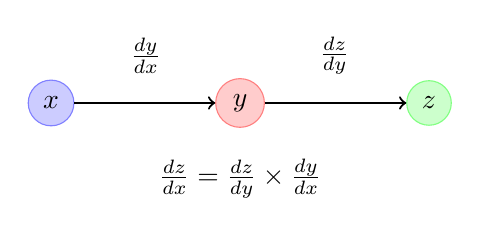
\begin{tikzpicture}[scale=1.2]
                % Chain of dependencies
                \node[circle, draw=blue!50, fill=blue!20] (x) at (0,0) {$x$};
                \node[circle, draw=red!50, fill=red!20] (y) at (2,0) {$y$};
                \node[circle, draw=green!50, fill=green!20] (z) at (4,0) {$z$};
                
                \draw[->, thick] (x) -- (y);
                \draw[->, thick] (y) -- (z);
                
                % Gradient annotations
                \node at (1,0.5) {$\frac{dy}{dx}$};
                \node at (3,0.5) {$\frac{dz}{dy}$};
                \node at (2,-0.8) {$\frac{dz}{dx} = \frac{dz}{dy} \times \frac{dy}{dx}$};
            \end{tikzpicture}
            \end{center}
    \end{columns}
\end{exampleblock}
\end{frame}

\begin{frame}{反向传播的详细步骤}

\begin{columns}
\column{0.5\textwidth}
    \begin{block}{步骤1:前向传播计算所有节点值}
    先正常计算每个节点的值,并保存起来。
    \end{block}

    \begin{block}{步骤2:从输出节点开始反向传播梯度}
    \begin{enumerate}
        \item 输出节点的梯度为1:$\frac{\partial L}{\partial L} = 1$
        \item 对每个节点,计算其对损失函数的梯度
        \item 使用链式法则将梯度反向传播
    \end{enumerate}
    \end{block}

\column{0.45\textwidth}
    \begin{exampleblock}{简单例子:$f(x,y) = (x+y) \times y$}
    假设$x=3, y=2$,我们要计算$\frac{\partial f}{\partial x}$和$\frac{\partial f}{\partial y}$:
    \begin{itemize}
        \item 前向传播:$u = x+y = 5$,$f = u \times y = 10$
        \item 反向传播:$\frac{\partial f}{\partial u} = y = 2$,$\frac{\partial f}{\partial y} = u = 5$
        \item 继续:$\frac{\partial f}{\partial x} = \frac{\partial f}{\partial u} \times \frac{\partial u}{\partial x} = 2 \times 1 = 2$
    \end{itemize}
    \end{exampleblock}
\end{columns}
\end{frame}

\begin{frame}{计算图示例:前向传播与反向传播}
    \begin{columns}
    \column{0.4\textwidth}
\begin{center}
\begin{tikzpicture}[
    node/.style={circle, draw=blue!50, fill=blue!20, minimum size=8mm},
    op/.style={circle, draw=red!50, fill=red!20, minimum size=8mm},
    label/.style={font=\small}
]
    % Forward pass values (top)
    \node at (3, 6) {\textcolor{blue}{前向传播值}};
    \node[node] (x) at (1,4.5) {$x=3$};
    \node[node] (y1) at (3,4.5) {$y_1=2$};
    \node[node] (y2) at (5,4.5) {$y_2=2$};
    \node[op] (plus) at (2,2.5) {$u=5$};
    \node[op] (times) at (4,2.5) {$f=10$};
    
    % Operation labels
    \node at (2,1.5) {\small{$u = x + y_1$}};
    \node at (4,1.5) {\small{$f = u \times y_2$}};

    % Edges for forward pass
    \draw[->, thick, blue] (x) -- node[above, sloped] {} (plus);
    \draw[->, thick, blue] (y1) -- node[above, sloped] {} (plus);
    \draw[->, thick, blue] (plus) -- node[above] {} (times);
    \draw[->, thick, blue] (y2) -- node[above, sloped] {} (times);
\end{tikzpicture}
\end{center}

\column{0.6\textwidth}
\begin{center}
\begin{tikzpicture}[
    node/.style={circle, draw=blue!50, fill=blue!20, minimum size=8mm},
    op/.style={circle, draw=red!50, fill=red!20, minimum size=8mm},
    label/.style={font=\small}
]
    % Backward pass gradients (bottom)
    \node at (3,3) {\textcolor{red}{反向传播梯度}};
    \node[node] (x2) at (1,1) {$\frac{\partial f}{\partial x}=2$};
    \node[node] (y1b) at (4,1) {$\frac{\partial f}{\partial y_1}=2$};
    \node[node] (y2b) at (7,1) {$\frac{\partial f}{\partial y_2}=5$};
    \node[op] (plusb) at (2.5,-1.5) {$\frac{\partial f}{\partial u}=2$};
    \node[op] (timesb) at (5.5,-1.5) {$\frac{\partial f}{\partial f}=1$};
    
    % Edges for backward pass
    \draw[<-, thick, red] (x2) -- node[below, sloped] {$\times 1$} (plusb);
    \draw[<-, thick, red] (y1b) -- node[below, sloped] {$\times 1$} (plusb);
    \draw[<-, thick, red] (plusb) -- node[below] {$\times 2$} (timesb);
    \draw[<-, thick, red] (y2b) -- node[below, sloped] {$\times 5$} (timesb);
    
    % Explanation
    \node at (3,-3) {\footnotesize{反向传播应用链式法则: $\frac{\partial f}{\partial x} = \frac{\partial f}{\partial u} \cdot \frac{\partial u}{\partial x}$}};
\end{tikzpicture}
\end{center}
\end{columns}
\end{frame}

\section{梯度下降}

\begin{frame}{为什么需要梯度下降?}
\begin{block}{核心问题}
我们已经知道如何计算梯度(偏导数),但\alert{如何利用这些信息来改进模型}?
\end{block}

\begin{columns}
    \column{0.5\textwidth}
\begin{exampleblock}{直觉思考}
\begin{itemize}
    \item 梯度告诉我们每个参数对误差的影响方向
    \item 正梯度:增加参数会增加误差
    \item 负梯度:增加参数会减小误差
    \item \alert{我们应该沿着梯度的反方向调整参数!}
\end{itemize}
\end{exampleblock}

    \column{0.4\textwidth}
\begin{center}
\begin{tikzpicture}[scale=1.2]
    % Function curve
    \draw[thick, domain=-2:2, smooth, variable=\x, blue] plot ({\x}, {0.5*\x*\x});
    
    % Points
    \fill[red] (1,0.5) circle (2pt);
    \fill[green] (-1,0.5) circle (2pt);
    
    % Gradient arrows
    \draw[->, thick, red] (1,0.5) -- (1.5,0.5);
    \draw[->, thick, green!70!black] (-1,0.5) -- (-1.5,0.5);
    
    % Labels
    \node at (1,-0.2) {正梯度};
    \node at (-1,-0.2) {负梯度};
    \node at (0,-0.8) {我们应该向左移动来减小函数值};
\end{tikzpicture}
\end{center}
\end{columns}
\end{frame}

\begin{frame}{梯度下降算法}

\begin{block}{基本思想}
\alert{沿着梯度的反方向}小步移动,逐步减小损失函数。
\end{block}

\begin{columns}
    \column{0.55\textwidth}
\begin{block}{数学表达}
对于参数$\theta$,更新规则是:
\[\theta_{\text{新}} = \theta_{\text{旧}} - \alpha \frac{\partial L}{\partial \theta}\]
其中:
\begin{itemize}
    \item $\alpha$是学习率(步长大小)
    \item $\frac{\partial L}{\partial \theta}$是损失函数对参数的梯度
    \item 减号表示沿着梯度的反方向移动
\end{itemize}
\end{block}

\column{0.4\textwidth}
\begin{exampleblock}{类比:下山}
\begin{itemize}
    \item 你站在山上,想下到最低点
    \item 观察周围最陡的方向(梯度)
    \item 沿着相反方向走一小步
    \item 重复这个过程直到到达谷底
\end{itemize}
\end{exampleblock}
\end{columns}
\end{frame}

\begin{frame}{梯度下降的完整过程}

\begin{columns}
    \column{0.6\textwidth}
        \begin{center}
        \begin{figure}[h]
            \includegraphics[width=1\textwidth]{images/gradient_descent.png}
        \end{figure}
        \end{center}
    \column{0.4\textwidth}
        \begin{block}{算法步骤}
            \begin{enumerate}
                \item 初始化参数$\theta$
                \item 计算当前梯度$\frac{\partial L}{\partial \theta}$
                \item 更新参数:$\theta = \theta - \alpha \frac{\partial L}{\partial \theta}$
                \item 重复步骤2-3直到收敛
            \end{enumerate}
        \end{block}
\end{columns}


\end{frame}

\begin{frame}{学习率的重要性}

\begin{columns}[t]
\column{0.45\textwidth}
\begin{block}{学习率太小}
\begin{itemize}
    \item 收敛速度很慢
    \item 需要很多迭代
    \item 可能陷入局部最优
\end{itemize}
\begin{center}
\begin{tikzpicture}[scale=0.6]
    \draw[->, thick, blue] (0,0) -- (1,0);
    \draw[->, thick, blue] (1,0) -- (1.3,0);
    \draw[->, thick, blue] (1.3,0) -- (1.5,0);
    \draw[->, thick, blue] (1.5,0) -- (1.6,0);
    \node at (0.8,-0.5) {小步移动};
\end{tikzpicture}
\end{center}
\end{block}

\column{0.45\textwidth}
\begin{block}{学习率太大}
\begin{itemize}
    \item 可能错过最优解
    \item 在最优解附近震荡
    \item 甚至发散(不收敛)
\end{itemize}
\begin{center}
\begin{tikzpicture}[scale=0.6]
    \draw[->, thick, red] (0,0) -- (2,0);
    \draw[->, thick, red] (2,0) -- (0,0);
    \draw[->, thick, red] (0,0) -- (2,0);
    \draw[->, thick, red] (2,0) -- (0,0);
    \node at (1,-0.5) {来回震荡};
\end{tikzpicture}
\end{center}
\end{block}
\end{columns}

\begin{alertblock}{选择合适的学习率}
\begin{itemize}
    \item 通常从0.01, 0.001等值开始尝试
    \item 可以随着训练逐渐减小
    \item 使用自适应方法(如Adam, RMSprop)
\end{itemize}
\end{alertblock}
\end{frame}

\section{综合实例}

\begin{frame}{完整例子:训练一个简单的模型}

\begin{block}{问题设定}
我们要训练一个模型$f(x) = wx + b$来拟合数据点$(2, 5)$。
\end{block}

\begin{columns}[t]
\column{0.5\textwidth}
\begin{block}{模型结构}
\begin{center}
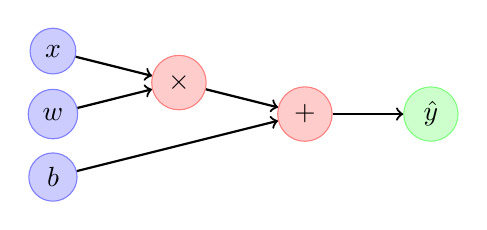
\begin{tikzpicture}[scale=0.8]
    \node[circle, draw=blue!50, fill=blue!20] (x) at (0,1) {$x$};
    \node[circle, draw=blue!50, fill=blue!20] (w) at (0,0) {$w$};
    \node[circle, draw=blue!50, fill=blue!20] (b) at (0,-1) {$b$};
    \node[circle, draw=red!50, fill=red!20] (mul) at (2,0.5) {$\times$};
    \node[circle, draw=red!50, fill=red!20] (add) at (4,0) {$+$};
    \node[circle, draw=green!50, fill=green!20] (y) at (6,0) {$\hat{y}$};
    
    \draw[->, thick] (x) -- (mul);
    \draw[->, thick] (w) -- (mul);
    \draw[->, thick] (mul) -- (add);
    \draw[->, thick] (b) -- (add);
    \draw[->, thick] (add) -- (y);
\end{tikzpicture}
\end{center}
\end{block}

\column{0.45\textwidth}
\begin{block}{训练步骤}
\begin{enumerate}
    \item 前向传播:计算$\hat{y}$
    \item 计算损失:$L = (\hat{y} - y)^2$
    \item 反向传播:计算梯度
    \item 梯度下降:更新$w$和$b$
    \item 重复直到收敛
\end{enumerate}
\end{block}
\end{columns}
\end{frame}

\begin{frame}{具体计算过程}
\begin{columns}
    \column{0.4\textwidth}
        \begin{block}{初始化}
        设$w=1, b=0$,学习率$\alpha=0.1$
        \end{block}
        \vspace{0.2cm}

        \begin{alertblock}{结果}
        新的参数:$w=2.2, b=0.6$,预测值更接近真实值了!
        \end{alertblock}
        \begin{block}{下一步}
        下一步,我们只需要重复这个过程,直到损失函数收敛到一个较小的值。
        \end{block}

    \column{0.55\textwidth}
        \begin{block}{第1轮迭代}
        \begin{enumerate}
            \item \alert{前向传播}:$x=2 \Rightarrow \hat{y} = 1\times 2 + 0 = 2$
            \item \alert{计算损失}:$L = (\hat{y} - y)^2 = (2-5)^2 = 9$
            \item \alert{反向传播}:
            \begin{itemize}
                \item $\frac{\partial L}{\partial \hat{y}} = 2(\hat{y} - y) = 2(2-5) = -6$
                \item $\frac{\partial L}{\partial w} = \frac{\partial L}{\partial \hat{y}} \times \frac{\partial \hat{y}}{\partial w} = -6 \times 2 = -12$
                \item $\frac{\partial L}{\partial b} = \frac{\partial L}{\partial \hat{y}} \times \frac{\partial \hat{y}}{\partial b} = -6 \times 1 = -6$
            \end{itemize}
            \item \alert{梯度下降}:
            \begin{itemize}
                \item $w_{\text{新}} = w - \alpha \frac{\partial L}{\partial w} = 1 - 0.1\times(-12) = 2.2$
                \item $b_{\text{新}} = b - \alpha \frac{\partial L}{\partial b} = 0 - 0.1\times(-6) = 0.6$
            \end{itemize}
        \end{enumerate}
        \end{block}
\end{columns}
\end{frame}

\section{总结与应用}

\begin{frame}{今天我们学到了什么?}

\begin{columns}
\column{0.45\textwidth}
\begin{block}{1. 计算图}
\begin{itemize}
    \item 将数学表达式可视化为图结构
    \item 清晰展示计算过程和依赖关系
    \item 为自动求导奠定基础
\end{itemize}
\end{block}

\column{0.45\textwidth}
\begin{block}{2. 反向传播}
\begin{itemize}
    \item 高效计算梯度的算法
    \item 基于链式法则从后向前传播梯度
    \item 让我们知道每个参数对误差的影响
\end{itemize}
\end{block}
\end{columns}

\begin{block}{3. 梯度下降}
\begin{itemize}
    \item 利用梯度信息优化参数
    \item 沿着负梯度方向小步前进
    \item 逐步减小损失函数,提高模型性能
\end{itemize}
\end{block}

\end{frame}

\begin{frame}{在深度学习中的应用}

\begin{block}{现代深度学习框架}
这些概念是所有深度学习框架的核心:

\begin{columns}[c]
\column{0.5\textwidth}
\begin{itemize}
    \item \textcolor{blue}{PyTorch}
    \item \textcolor{orange}{TensorFlow}
    \item \textcolor{red}{JAX}
    \item \textcolor{teal}{MXNet}
\end{itemize}

\column{0.5\textwidth}
\begin{itemize}
    \item 自动构建计算图
    \item 自动微分(反向传播)
    \item 内置优化器(梯度下降变体)
    \item 让我们专注于模型设计
\end{itemize}
\end{columns}
\end{block}

\begin{exampleblock}{实际应用}
\begin{itemize}
    \item 计算机视觉:图像分类、目标检测
    \item 自然语言处理:机器翻译、文本生成
    \item 语音识别、推荐系统、游戏AI
    \item 科学计算、医疗诊断、金融预测
\end{itemize}
\end{exampleblock}
\end{frame}

\begin{frame}{下一步学习建议}

\begin{block}{巩固基础}
\begin{enumerate}
    \item 动手实现简单的神经网络
    \item 使用PyTorch或TensorFlow练习
    \item 可视化梯度流动和参数更新
    \item 调试和优化训练过程
\end{enumerate}
\end{block}

\begin{block}{深入拓展}
\begin{itemize}
    \item 不同类型的优化器(Adam, RMSprop)
    \item 梯度消失和梯度爆炸问题
    \item 更复杂的网络结构(CNN, RNN, Transformer)
    \item 正则化技术和训练技巧
\end{itemize}
\end{block}
\end{frame}

\begin{frame}{谢谢大家!}
\begin{center}
\Large
\textcolor{myblue}{谢谢大家!}\\
\vspace{0.3cm}
\large
\textcolor{mygreen}{有问题欢迎提问!}
\end{center}
\end{frame}

\end{document}